% ==========================================================================
% Long Data -- City of Boulder Emerging Technologies Taskforce
% October 21, 2026, 4:00-5:30pm (virtual); a talk of up to 15 minutes on
% "Emerging technology for improved access to and use of historic
% documentation"
% Build:  latexmk -pdf 2026-10-21-ett.tex   (from this folder; run twice)
% Format: the INFO 4617 course decks (Gotham theme; preamble in common/)
% Notes:  latexmk -pdf -jobname=2026-10-21-ett-notes \
%           -usepretex='\def\shownotes{}' 2026-10-21-ett.tex
% Each frame's speaker note names the taskforce prompt it answers.
% ==========================================================================
\documentclass[9pt,aspectratio=169]{beamer}
% Resolve the theme and preamble in common/ when compiling from this folder
\makeatletter\def\input@path{{common/}}\makeatother
\input{preamble}
\usepackage{array}  % for the appendix table's p{} columns

% Speaker notes: the notes build defines \shownotes (see README.md). For
% notes beside each slide instead, use show notes on second screen=right.
\ifdefined\shownotes\setbeameroption{show notes}\fi

\title[Long Data]{{\Huge Long Data}}
\subtitle{Emerging technology for improved access to and use of historic documentation \\ Emerging Technologies Taskforce · City of Boulder}
\author[Keegan]{\textbf{Brian C. Keegan, Ph.D.} \\ Associate Professor, Department of Information Science \\ University of Colorado Boulder}
\date{October 21, 2026}

\begin{document}

\maketitle

% =========================================================================
\section{Long data}
% =========================================================================

\begin{frame}{Long data}
    Big data is wide and shallow: many records, short history

    \medskip

    Municipal data is narrow and deep: one jurisdiction, recorded continuously across generations

    \medskip

    Boulder incorporated on November 4, 1871, and adopted its home rule charter on October 30, 1917. The charter has been amended ever since

    \bigskip

    \begin{alertblock}{Consequences}
        The city's records run 154 years deep. Nothing else the city owns covers that span
    \end{alertblock}

    \bottomcite{The term is Samuel Arbesman's: ``Stop Hyping Big Data and Start Paying Attention to `Long Data','' \textit{Wired}, January 29, 2013}

    \note{Taskforce prompt: overview of the topic. Land the reframe before anything technical. Everyone in the room has heard a big-data pitch. Nobody has heard this one.}
\end{frame}

\begin{frame}{Retrieval fits long data}
    Most technology pitched to cities is built for big data: scale, throughput, statistical power

    \medskip

    Retrieval, knowledge graphs, and agent harnesses fit long data better: a small corpus, strict provenance, and the same people, places, and laws named differently across decades

    \medskip

    Document intelligence changed the price of reading. An accurate machine reading of a scanned page now costs under a cent

    \bigskip

    \begin{block}{The requirement}
        Provenance: find the 1974 staff memorandum, and say which page it is on
    \end{block}

    \begin{alertblock}{Consequences}
        What stays expensive is knowing where to look and checking what the machine read
    \end{alertblock}

    \note{Taskforce prompts: overview; what do we know today. The price-of-reading line is the hinge for the middle of the talk. The sprints and the revenue demo are the evidence for it.}
\end{frame}

\begin{frame}{Erosion, enclosure, exemption}
    The record can fail without anyone hiding anything

    \medskip

    \begin{description}\small
        \item[Erosion.] The record degrades through ordinary operations. The hotline archive splits at a 2023 server migration. Attachments were severed from the messages that cite them. OpenColorado, the shared repository for Colorado jurisdictions, has been retired
        \item[Enclosure.] Documents stay public while the routes to them are fenced: opaque numeric identifiers, automated access disallowed, export ceilings, custody split across four custodians
        \item[Exemption.] What never enters the record. Deliberation that moves to a phone call. Material never digitized, which is functionally nonexistent
    \end{description}

    \medskip

    \begin{block}{Each has a counter}
        Ownership answers erosion, openness answers enclosure, and oversight answers exemption
    \end{block}

    \note{Taskforce prompt: overview. These three are the analytic for the whole talk and for whatever the taskforce looks at next. Do not rush them.}
\end{frame}

\begin{frame}{The city charter}
    The Charter of the City of Boulder, adopted October 30, 1917, sits in the city's records portal

    \medskip

    The portal disallows automated access and addresses documents by opaque integers

    \medskip

    The same charter is a free download from the university law library: item 31 in its collection of historical Colorado municipal codes

    \bigskip

    \begin{alertblock}{Consequences}
        The city scanned the charter; the law library made it downloadable. The law library is a partner the city already has, and its collection shows what the work looks like
    \end{alertblock}

    \note{Taskforce prompts: what do we know today; examples. Erosion and enclosure in one object. Frame it as an offer, not a complaint.}
\end{frame}

% =========================================================================
\section{What we know today}
% =========================================================================

\begin{frame}{What the city holds}
    \begin{columns}[T]
        \begin{column}{0.47\textwidth}
            \begin{itemize}\small
                \item \textbf{Legislative:} ordinances, minutes, charter and code versions
                \item \textbf{Deliberative:} recordings, hotline, staff memoranda
                \item \textbf{Land:} permits, plats, variances, zoning, annexations
                \item \textbf{Planning and fiscal:} comprehensive plans, capital programs, budget books
                \item \textbf{Spatial:} GIS vintages, aerial series, floodplain maps
                \item \textbf{Electoral:} ballot measures, results, campaign finance
            \end{itemize}
        \end{column}
        \begin{column}{0.48\textwidth}
            \small
            \begin{tabular}{lll}
                \toprule
                \textbf{Tier} & \textbf{Machine-readable} & \textbf{Extent} \\
                \midrule
                Digital, text layer & Yes & Small \\
                Scanned, no text    & No  & Large \\
                Paper, film, AV     & No  & Unknown \\
                \bottomrule
            \end{tabular}

            \medskip

            The largest untapped tier is audio: decades of council and board deliberation

            \medskip

            Adopted text records the decision. Deliberation records the reason
        \end{column}
    \end{columns}

    \bigskip

    \begin{alertblock}{Consequences}
        Nobody can yet say how the holdings split across these three tiers, and every cost estimate depends on that split
    \end{alertblock}

    \note{Taskforce prompt: what do we know today. Read the left column at pace; its value is cumulative weight. If asked where to start: an inventory, not a procurement.}
\end{frame}

\begin{frame}{Two liberation sprints}
    \begin{columns}[T]
        \begin{column}{0.48\textwidth}
            \begin{block}{City budget books, 2002--2027}
                \small 34 PDFs and 10,843 pages from the city's records portal. Six volumes, 1,651 pages, have no text layer at all. The budget portal offers no public data endpoint

                \medskip

                \textbf{Result:} 450 figures across 26 years, each traced to its source document
            \end{block}
        \end{column}
        \begin{column}{0.48\textwidth}
            \begin{block}{State school yearbooks, 1986--1999}
                \small The scans' built-in text layer recovered 3.9\% of one table's cells. Accurate OCR read the rest at 0.75 cents a page, about \$5 for fourteen volumes

                \medskip

                \textbf{Result:} 1,267 of 1,269 figures read twice agree exactly
            \end{block}
        \end{column}
    \end{columns}

    \bigskip

    \begin{alertblock}{Consequences}
        Reading the pages cost a few dollars. The time went to finding the right pages, checking every figure, and naming every gap
    \end{alertblock}

    \bottomcite{Source: Charting Boulder repository, budget-history and alternatives folders}

    \note{Taskforce prompt: what do we know today. First person here: I did this on my own time for a newspaper column. If one person can do it for a column, the city can do it for the public record.}
\end{frame}

% -------------------------------------------------------------------------
% Demo: Web Data Science, Chapter 9, "Case Study: Boulder Revenue Reports"
% -------------------------------------------------------------------------

\begin{frame}[fragile]{The city's records portal}
    \begin{columns}[T]
        \begin{column}{0.5\textwidth}
            The Finance Department files a year-end revenue report in the city's records portal

            \medskip

            The folder's page arrives saying ``Loading...''; a script fills in the list

            \medskip

            Behind the list is one request. It sends the folder's number and gets back a structured listing

            \medskip

            Each download is checked before it is read. A PDF starts with the bytes \texttt{\%PDF-}; for a scanned record, the same address answers with an empty file
        \end{column}
        \begin{column}{0.47\textwidth}
            \begin{block}{Program output}
\begin{lstlisting}[language={},basicstyle=\ttfamily\scriptsize]
\Central Records\Finance\Reports\Revenue Reports
7 entries
194346 2021 (folder)
194359 2022 (folder)
194372 2023 (folder)
194385 2024 (folder)
194398 Revenue Report 2018 (15 pages)
194399 Revenue Report 2019 (14 pages)
194400 Revenue Report 2020 (16 pages)

application/pdf 723920 b'%PDF-'
\end{lstlisting}
            \end{block}
            {\scriptsize Chapter 9's code, October 2026: the folder's listing, then the December 2024 report's type, size, and first bytes}
        \end{column}
    \end{columns}

    \medskip

    \begin{alertblock}{Consequences}
        Each report takes its own request. On October 6, 2026, the server stopped answering after 13 to 17 requests in a row and answered again after a five-minute pause
    \end{alertblock}

    \note{Taskforce prompt: what do we know today. This is a textbook chapter my students work through: retrieving and reading the city's own reports. Say "records portal"; the taskforce asked us not to comment on specific providers. Code is in the appendix.}
\end{frame}

\begin{frame}[fragile]{Reading one report}
    \begin{columns}[T]
        \begin{column}{0.54\textwidth}
            Each report opens with a summary table of sales and use tax, the city's largest source of revenue, for this year and the year before

            \medskip

            The table is on page 2 of every report except 2020's, which opens with a restatement letter. So the code finds the page by its first sentence, not its number

            \medskip

            It reads the totals row by its position on the page, then checks it: this year minus last year must equal the change the report prints
        \end{column}
        \begin{column}{0.42\textwidth}
            \begin{block}{Program output, 2018 report}
\begin{lstlisting}[language={},basicstyle=\ttfamily\scriptsize]
('2017', '2018')
['$134,538,892', '$140,648,710',
 '$6,109,818', '4.54%']

14 figures from 7 reports;
every change column checks
\end{lstlisting}
            \end{block}
            {\scriptsize The heading's two years, then the totals row: last year, this year, the change in dollars, the change in percent}
        \end{column}
    \end{columns}

    \bigskip

    \begin{alertblock}{Consequences}
        Six years are printed in two reports each. Five agree to the dollar. The two printings of 2018 differ by \$38,959, and neither report says why
    \end{alertblock}

    \note{Taskforce prompt: what do we know today. A reading that can't be checked against the document's own arithmetic is a guess. The series uses each year's latest printing, and says so.}
\end{frame}

\begin{frame}{Eight years of sales and use tax}
    \centering
    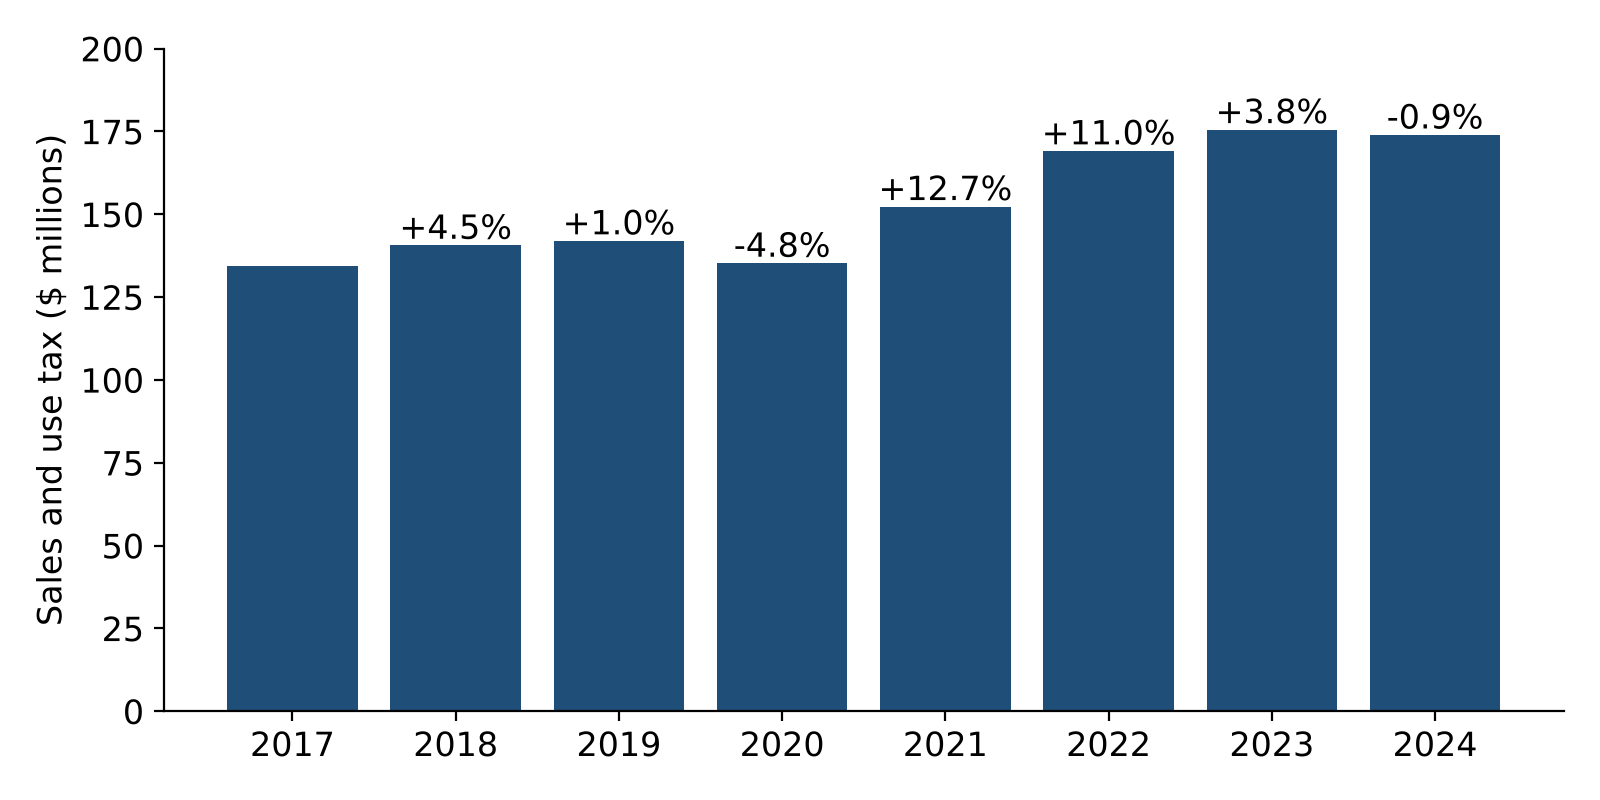
\includegraphics[width=0.62\textwidth]{img/sales-use-tax.png}

    \raggedright\scriptsize
    Total sales and use tax, 2017--2024, read from the summary tables of seven year-end revenue reports. Each year uses its latest printing. Dollars of each year, not adjusted for inflation

    \medskip

    \begin{alertblock}{Consequences}
        \small Down 4.76\% in 2020, up more than 10\% in both 2021 and 2022, down 0.92\% in 2024. Every figure traces to a page of a named report
    \end{alertblock}

    \bottomcite{Keegan, \textit{Web Data Science}, Chapter 9, ``Case Study: Boulder Revenue Reports'' (github.com/cuinfoscience/Web-Data-Science-Book); the city's revenue reports, 2018--2024, retrieved October 6, 2026}

    \note{Taskforce prompt: what do we know today. Two requests per report, a page found by its wording, one row read by position, one arithmetic check. That is the whole method, and it already works on the city's records.}
\end{frame}

\begin{frame}{Archive, derived, and retrieval layers}
    \begin{block}{Archive layer}
        \small Originals exactly as received and never edited. Each carries a checksum, its source URL, and its retrieval date
    \end{block}
    \begin{block}{Derived layer}
        \small Text and tables extracted from the originals. Every value names its source document, machine readings are marked as such, each document's totals are checked against its own parts (the revenue reports' change column is one such check), and a failed check stops the build. Gaps are named, never filled
    \end{block}
    \begin{block}{Retrieval layer}
        \small Search, pipelines, and agents. Every answer cites back down to a document and page
    \end{block}

    \medskip

    \small Each rule answers a failure. OCR invented values from percentages and read a bar chart as numbers; the budget book's own arithmetic caught both. A pipeline once wrote nine copies of fourteen years of records, and every total still looked right

    \note{Taskforce prompt: what would the city need to do. This is the argument that the data lake needs a spine. Retrieval without the two layers beneath it is a fluent guess.}
\end{frame}

% =========================================================================
\section{Implications for the city}
% =========================================================================

\begin{frame}{What council asks about}
    \centering
    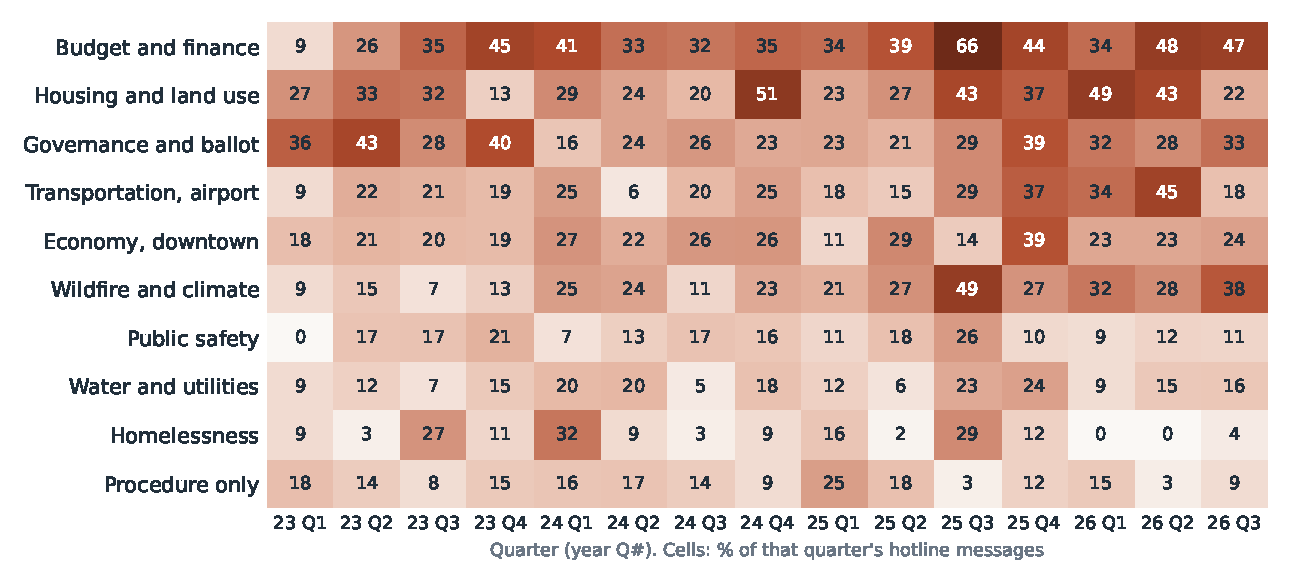
\includegraphics[width=\textwidth,height=0.62\textheight,keepaspectratio]{img/deck-themes-by-quarter.pdf}

    \raggedright\small
    Budget runs through every quarter. Wildfire and climate roughly tripled their share after 2023. Homelessness spikes, then nearly vanishes in 2026

    \bottomcite{City of Boulder open data, ``Emails to the City Council Hotline'' (CC0), March 2, 2023 to September 15, 2026: 779 hotline-list messages, classified by keyword}

    \note{Taskforce prompt: implications for the city. All 779 hotline-list messages, classified by keyword. The primary theme matched in about 22 of 25 messages I checked by hand; secondary labels are generous on long messages.}
\end{frame}

\begin{frame}{The council hotline}
    Since March 2023: 779 hotline messages, 207 council question posts holding about 1,090 question marks, and 142 staff responses. I coded a random 40 of those responses

    \medskip

    \begin{center}
        \small
        \begin{tabular}{lr}
            \toprule
            \textbf{What the answer required} & \textbf{Responses} \\
            \midrule
            Procedural: a resend, a logistics note, a transmittal & 10 \\
            Lookup: the answer already sits in a packet, memo, ordinance, or dataset & 10 \\
            Mixed: a factual scaffold from the record, plus judgment & 14 \\
            Judgment: new analysis or a policy position & 6 \\
            \bottomrule
        \end{tabular}
    \end{center}

    \medskip

    \begin{alertblock}{Consequences}
        A third of the substantive answers were lookups. One in five needed judgment that no record holds
    \end{alertblock}

    \bottomcite{One coder, n = 40. One set of wildfire answers credits more than twenty staff. Nearly every message is flagged as carrying an attachment; none of the attachments are in the published dataset}

    \note{Taskforce prompt: implications for the city. The right verb is drafted with citations. Answers to elected officials go out under a staff member's name, and should. Script and coding sheet are public; offer them.}
\end{frame}

\begin{frame}{What to liberate first}
    \begin{columns}[T]
        \begin{column}{0.44\textwidth}
            {\scriptsize Records needed to answer: share of 349 council questions and staff responses}

            \smallskip

            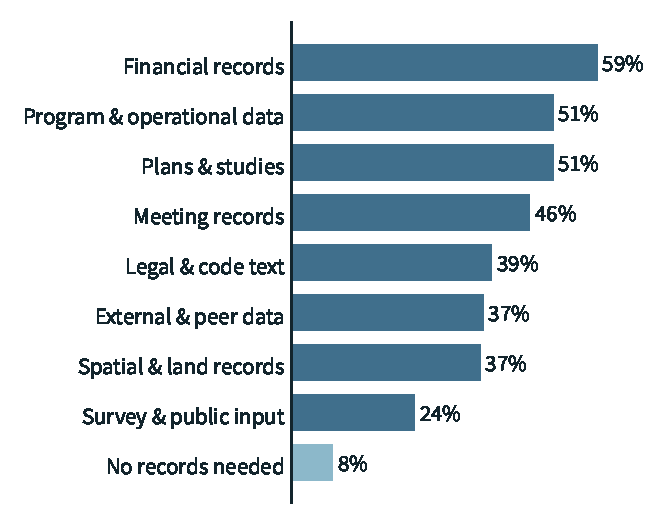
\includegraphics[width=0.92\textwidth]{img/deck-records-needed.pdf}

            \medskip

            \small Financial records are needed for three in five answers, and in every theme
        \end{column}
        \begin{column}{0.52\textwidth}
            \footnotesize
            \textbf{Start now} --- high demand, low privacy risk
            \begin{itemize}\setlength\itemsep{0pt}
                \item Budget books, revenue reports, audits
                \item Council packets and staff memoranda
                \item Ordinances, resolutions, and code versions
            \end{itemize}
            \textbf{Next} --- high research value, higher cost
            \begin{itemize}\setlength\itemsep{0pt}
                \item Minutes and meeting recordings
                \item Plans and consultant studies
                \item Board and commission appointments
                \item Program year-end reports
            \end{itemize}
            \textbf{With screening} --- personal information
            \begin{itemize}\setlength\itemsep{0pt}
                \item Permits and land records
                \item Hotline mail and public comment
            \end{itemize}
        \end{column}
    \end{columns}

    \note{Taskforce prompts: implications for the city; key opportunities. The ranking weighs three things: how often council needs the record, how far back it runs, and how much personal information it carries. Appointments are small and cheap, and they supply the identity key: who served on what, when. Detail is in the appendix.}
\end{frame}

% =========================================================================
\section{Opportunities and obligations}
% =========================================================================

\begin{frame}{Accessibility remediation}
    Scanned image documents are unreadable to screen readers

    \medskip

    Six volumes of the city's own budget books, 1,651 pages, have no text layer at all

    \medskip

    Federal accessibility obligations require the text layer whether or not the city builds anything on top of it

    \bigskip

    \begin{alertblock}{Consequences}
        The spending is already owed. The choice is whether it produces a reusable public corpus or a pile of remediated documents
    \end{alertblock}

    \note{Taskforce prompt: key opportunities and risks. Lead with this in any conversation involving money. It is the only commitment with an external deadline attached.}
\end{frame}

\begin{frame}{Vendor lock-in}
    \begin{enumerate}\setlength\itemsep{3pt}
        \item \textbf{Stable, resolvable identifiers for every document.} Cheap, and every later step needs them
        \item \textbf{Bulk export and programmatic access as contract terms} at renewal. Twenty-six years of budget history had to be rebuilt from PDFs because the budget portal offers no data endpoint
        \item \textbf{Open document standards} for legislative markup, scanned images, and preservation metadata. Vendors become interchangeable, with no need to win an argument about any one of them
        \item \textbf{The licensing the city already uses}, extended to its documents
    \end{enumerate}

    \bigskip

    \begin{alertblock}{Consequences}
        The open data catalog is already published under a license that permits copying, adaptation, and redistribution without attribution. The license stops at the records portal
    \end{alertblock}

    \note{Taskforce prompt: what would the city need to do. Item 4 is the disarming one: consistency with the city's own practice, not a new philosophy. Keep it general; no vendor names.}
\end{frame}

\begin{frame}{Community capacity}
    The open data program already partners with local civic data groups

    \medskip

    A local civic-tech group already maintains a directory of roughly a hundred Boulder datasets

    \medskip

    The law library already digitized the charter

    \medskip

    I rebuilt 26 years of the city's budget history from its own PDFs for a newspaper column

    \medskip

    A published corpus becomes a data lake that staff, partners, pipelines, and agents can all draw from

    \bigskip

    \begin{alertblock}{Consequences}
        The constraint is staff time. Publishing a corpus turns outside interest into capacity the city never has to hire, and it is the only one of these commitments that pays back without a procurement
    \end{alertblock}

    \note{Taskforce prompt: key opportunities. Name the groups if the room knows them. This is also the answer to ``we don't have the staff for this.''}
\end{frame}

\begin{frame}{Examples from other sectors}
    \begin{itemize}\setlength\itemsep{2pt}
        \item National legislative databases publish point-in-time versions of law, so a reader can see what was in force on a given date
        \item Federal programs publish legislative data as bulk downloads rather than only through a search box
        \item National archives run text and handwriting recognition across historical holdings at scale
        \item Heritage institutions use volunteer transcription as a capacity model requiring no procurement
        \item Court systems publish structured opinions with stable citations
        \item Newsrooms build document-mining pipelines for large records releases
    \end{itemize}

    \bigskip

    \begin{alertblock}{Consequences}
        Each of them publishes the corpus and treats the search interface as replaceable
    \end{alertblock}

    \note{Taskforce prompt: relevant examples, kept general. If someone asks which vendor does this: every example here is an institution or a sector, not a product.}
\end{frame}

% =========================================================================
\section{Outlook and risks}
% =========================================================================

\begin{frame}{What happens next, and why I might be wrong}
    \begin{itemize}\setlength\itemsep{3pt}
        \item Context windows may grow enough that retrieval architecture becomes unnecessary. The provenance requirement survives either way, which is why I anchored on it
        \item The binding constraint has already moved from compute to verification and permission: retention schedules, legal review, metadata quality. None of those follow a hardware curve
        \item Multi-step agentic research on legal precedent is unmeasured on municipal corpora. Errors compound, and nothing surfaces them
        \item \textbf{Demand may be low.} The hotline suggests otherwise, but one coder and forty messages is thin evidence
        \item The most likely failure is not technical: a multi-year project dies on a budget cycle and one departure
    \end{itemize}

    \note{Taskforce prompt: what do we think will happen, and why might we be wrong. Say the demand bullet flat. It is the strongest objection to my own recommendation and the room should hear me make it first.}
\end{frame}

\begin{frame}{Three kinds of holdings}
    \begin{description}
        \item[Already data.] Published, licensed, documented: the open data catalog
        \item[Could become data.] The archives, the budget books, the hotline and its attachments, the recordings, the backlog. The technology argument is about these
        \item[Shouldn't become data.] The category with no policy, because nobody writes one until the corpus already exists
    \end{description}

    \bigskip

    \begin{alertblock}{Consequences}
        The city can sort each holding into one of the three on purpose. A holding left unsorted gets sorted by whoever builds on it first
    \end{alertblock}

    \note{Taskforce prompts: key risks; what would the city need to do. This is the deliverable. Offer to circulate this slide alone.}
\end{frame}

\begin{frame}{Shouldn't become data}
    Candidates: surveillance feeds, individual utility and recreation customer records, code enforcement complaints naming residents, protective-order addresses, records carrying victim and juvenile information

    \medskip

    \begin{itemize}
        \item The argument is about \textbf{aggregation, not disclosure}. Records obligations do not change. What changes is whether the city builds the index that makes assembling a dossier trivial
        \item Practical obscurity is a protection nobody wrote down. Retrieval removes it unless someone decides to keep it
        \item Precedent exists: the published hotline dataset already replaces contact details with one-way hashes
    \end{itemize}

    \medskip

    \begin{block}{Exemption, used on purpose}
        Exemption is the force to resist for the first two kinds of holdings and the mechanism to use for the third. Scoped that way, it makes the other two safe to build
    \end{block}

    \note{Taskforce prompts: key risks; mitigation. Guard against being heard as anti-transparency. Say the aggregation/disclosure distinction twice if needed.}
\end{frame}

\begin{frame}{Would impacts fall unevenly in our community?}
    \begin{enumerate}\setlength\itemsep{4pt}
        \item \textbf{Digitization order becomes citation order.} What is not scanned is functionally nonexistent to a researcher or an analyst, and the least-digitized holdings are disproportionately those of the least powerful
        \item \textbf{Text recognition fails unevenly.} It fails worst on old, handwritten, tabular, and non-English material, so retrieval quality degrades along the same axis as the equity concern
        \item \textbf{Aggregation lands unevenly.} It falls hardest on residents with the most contact with enforcement systems
    \end{enumerate}

    \bigskip

    \begin{alertblock}{Consequences}
        These harms fall on the residents least able to object, through records the city already holds, whether or not anyone intends them. They should set which holdings are digitized first
    \end{alertblock}

    \note{Taskforce prompt: would impacts be disproportionately felt in our community. Do not soften this into a caveat. It is a sequencing constraint: it should change which holdings are digitized first.}
\end{frame}

\begin{frame}{Key takeaways}
    \begin{enumerate}\setlength\itemsep{4pt}
        \item The city's records are \textbf{long data}: one jurisdiction, 154 years
        \item Machine reading is cheap; \textbf{finding and checking} the right pages is the work
        \item Nobody knows how much of the backlog a machine can read. \textbf{An inventory} comes before a procurement
        \item \textbf{Provenance first}: every answer cites a document and a page
        \item Sort each holding: already data, could become data, \textbf{shouldn't become data}
    \end{enumerate}

    \bigskip

    \begin{alertblock}{The test}
        The first proposal that arrives with a demonstration attached: which of the three kinds is its corpus, and which layer is it selling?
    \end{alertblock}

    \note{Taskforce prompt: what would the city need to do. Ten minutes in a browser and two sprints are not an audit. The finding I hold with the most confidence is the one we cannot close from in here: nobody knows the size of the backlog. If we cannot answer the test's two questions, the demonstration is doing the sorting for us. What the city still holds after a vendor leaves is a choice available now, while it is cheap.}
\end{frame}

% =========================================================================
% Appendix: unnumbered, so the footer counts only the talk's own frames.
% (Gotham's \appendix adds a part page and a contents page, so it isn't used.)
% =========================================================================

\setbeamertemplate{footline}{
  \begin{beamercolorbox}[wd=\paperwidth,ht=2.5ex,dp=1ex,right]{footline}
    {\footnotesize Appendix}
    \hspace*{2ex}
  \end{beamercolorbox}
}

\begin{frame}[noframenumbering]{Appendix: record priorities in detail}
    \scriptsize\renewcommand{\arraystretch}{1.05}
    \begin{tabular}{>{\raggedright\arraybackslash}p{0.24\textwidth}>{\raggedright\arraybackslash}p{0.25\textwidth}>{\raggedright\arraybackslash}p{0.33\textwidth}l}
        \toprule
        \textbf{Record} & \textbf{Serves} & \textbf{What we know of its state} & \textbf{Tier} \\
        \midrule
        Budget books & Financial questions; 26-year series & 2002--2027 in the records portal; 1,651 pages lack text & Start \\
        Revenue reports & Financial questions & In the records portal, 2018--2024 (chapter 9); also sent as hotline attachments, which are not in the dataset & Start \\
        Council packets and memoranda & Meeting records; plans; the answers themselves & Recent years in the agenda system; depth unknown & Start \\
        Ordinances, resolutions, code versions & Legal text; the time key & Current code with a hosted vendor; history in the records portal & Start \\
        Minutes and recordings & Deliberation and intent & Unknown; needs inventory & Next \\
        Plans and consultant studies & Plans and studies & BVCP: 15 editions converted, 1977--2026 & Next \\
        Board and commission appointments & The identity key & Announced on the hotline; rosters unknown & Next \\
        Program year-end reports & Operational data & Some sent as hotline attachments & Next \\
        Permits and land records & The place key & Department systems; custody split & Screen \\
        Hotline and public comment & Demand signal; deliberation & 885 records since March 2023; contact details hashed & Screen \\
        \bottomrule
    \end{tabular}

    \note{``Unknown'' is a finding: each one is a line on the inventory.}
\end{frame}

\begin{frame}[noframenumbering]{Appendix: which records each theme depends on}
    \centering
    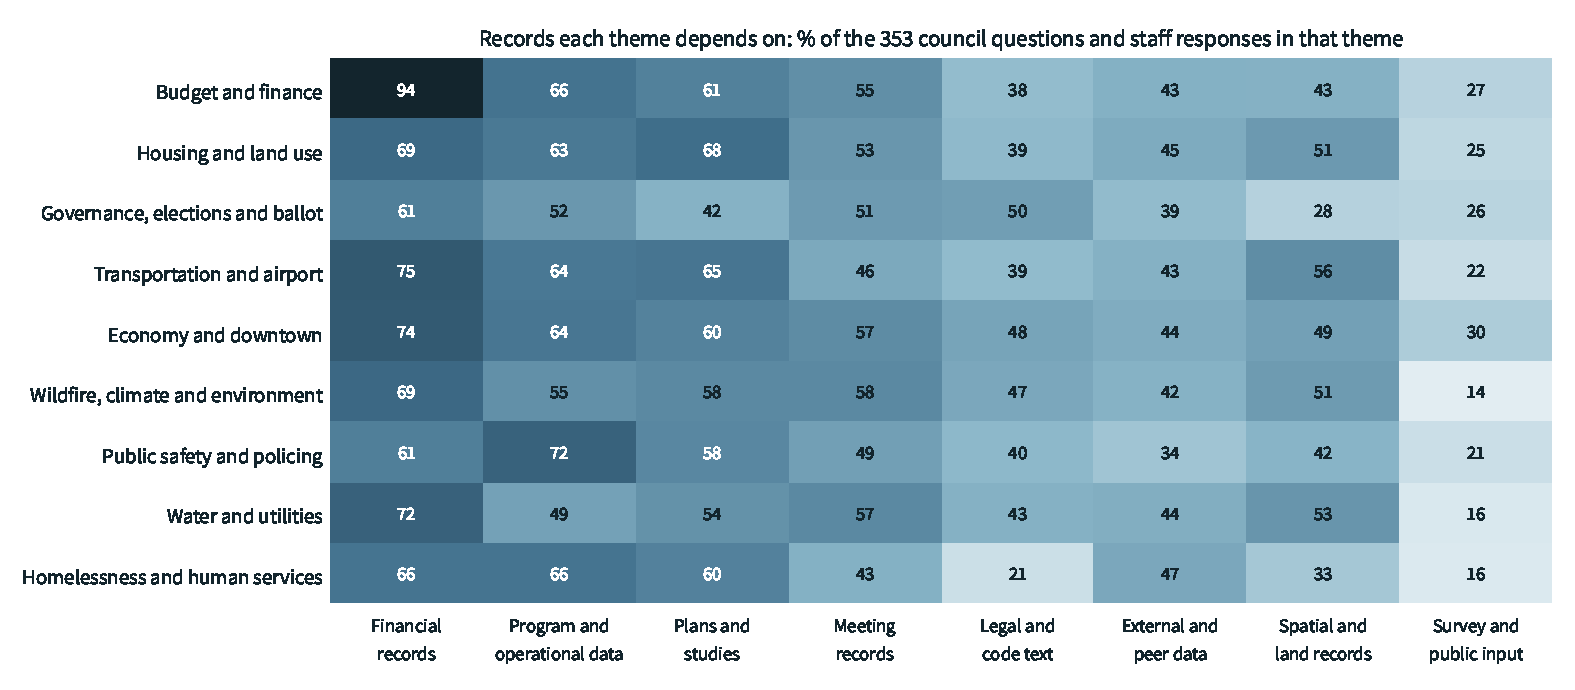
\includegraphics[width=\textwidth,height=0.62\textheight,keepaspectratio]{img/hotline-theme-by-records.pdf}

    \raggedright\small
    Financial records sit above 60\% in every theme. The spread across columns is flat: most answers need several kinds of record at once
\end{frame}

\begin{frame}[noframenumbering]{Appendix: hotline method}
    \begin{itemize}\small\setlength\itemsep{3pt}
        \item \textbf{Source.} City open data layer ``Emails to the City Council Hotline'' (CC0): 885 records, March 2, 2023 to September 15, 2026. 106 are off-list or unsolicited mail; 779 remain
        \item \textbf{Text.} Subject plus the authored top of each message. Quoted thread text, signatures, addresses, hashed contact tokens, and legal boilerplate are removed first
        \item \textbf{Themes.} Nine keyword dictionaries, multi-label, on all 779 messages
        \item \textbf{Records needed.} Eight dictionaries, applied only to the 349 council questions and staff responses, where a need is real
        \item \textbf{Checks.} Primary theme matched in about 22 of 25 messages read by hand. The lookup, mixed, and judgment coding on the hotline frame is a separate hand-coded sample of 40
        \item \textbf{Limits.} Keywords see words, not intent. Attachments, where many answers live, are not in the data
    \end{itemize}

    \bottomcite{Code, dictionaries, and outputs: \texttt{code/hotline\_provocation.py}, \texttt{code/hotline\_themes.py}}
\end{frame}

\begin{frame}[fragile,noframenumbering]{Appendix: getting a report from the records portal}
\begin{lstlisting}
import requests, time
# PORTAL, LISTING, and DOWNLOAD hold the portal's addresses; chapter 9 gives them in full
HEADERS = {"User-Agent": "WebDataScience/1.0 (your-email@colorado.edu)"}
# The folder's listing: the request the folder page itself sends (194345 is Revenue Reports)
body = {"folderId": 194345, "getNewListing": True, "start": 0, "end": 100}
response = requests.post(PORTAL + LISTING, json=body, headers=HEADERS, timeout=60, verify=bundle)
for entry in response.json()["data"]["results"]:
    print(entry["entryId"], entry["name"])

time.sleep(30)  # wait between requests to the city's server
response = requests.get(PORTAL + DOWNLOAD.format(docid=194397), headers=HEADERS, timeout=120, verify=bundle)
print(response.headers["Content-Type"], len(response.content), response.content[:5])
# application/pdf 723920 b'%PDF-'
\end{lstlisting}

    \small \texttt{bundle} is the certificate file the book provides: the city's server is set up in a way browsers forgive and Python doesn't. Chapter 9 also sends the request fields the page adds

    \bottomcite{Condensed from Keegan, \textit{Web Data Science}, Chapter 9, ``Getting the Files'' (github.com/cuinfoscience/Web-Data-Science-Book)}
\end{frame}

\begin{frame}[fragile,noframenumbering]{Appendix: reading and checking the totals row}
\begin{lstlisting}
import pdfplumber

def row_words(page, label):
    """Return the words to the right of label, on the line where label is."""
    found = page.search(label)[0]  # where the label sits on the page, in points
    line = page.crop((0, found["top"] - 1, page.width, found["bottom"] + 1))
    return [w["text"] for w in line.extract_words() if w["x0"] > found["x1"]]

for name in REPORTS:
    with pdfplumber.open(name) as pdf:
        page = find_summary_page(pdf)  # the page whose text includes "This report provides"
        earlier, this, change = [to_number(t) for t in row_words(page, "Total Sales and Use Tax")[:3]]
    if this - earlier != change:  # the report's own change column is the check
        print(f"{name}: {this:,} - {earlier:,} is not {change:,}")
# (nothing printed: every change column checks)
\end{lstlisting}

    \small \texttt{to\_number} turns ``\$134,538,892'' or ``(1,145,528)'' into an integer; accountants write a negative number in parentheses

    \bottomcite{Condensed from Keegan, \textit{Web Data Science}, Chapter 9, ``Reading the Totals Row by Position'' (github.com/cuinfoscience/Web-Data-Science-Book)}
\end{frame}

\end{document}
